\documentclass[12pt]{article}

\usepackage[slovene, english]{babel} 


\usepackage[utf8]{inputenc}
\usepackage[T1]{fontenc}
\usepackage{lmodern}
\usepackage{amsmath}
\usepackage{verbatim}
\usepackage{amssymb}
\usepackage{mathtools}
\usepackage{enumerate}
\usepackage{url}
\usepackage{hyperref}
\usepackage{graphicx}
\usepackage{float}

\setlength{\parindent}{0pt}

\begin{document}

\begin{center}

\Huge{\textbf{Homework MCMC}} \\
\textsc{\Large{Andraž De Luisa}} \\

\end{center}

\begin{enumerate}[A)]

    \item $X \sim N(0, 1), ~ f(x) = 10 \exp{(-5 (x-3)^4)}$
        \begin{enumerate}[1.]
            \item $I = E_X[f(x)] = \int_{-\infty}^{\infty} f(x) p(x) dx = 0.089$, with absolute error $< 2e-5$, where $p(x)$ is the standard normal distribution density.
            \item Monte-Carlo approximation (100 samples): $I = 0.062$ with $SE = 0.053$.
            \item Repeat the Monte-Carlo approximation 1000 times: for each iteration we construct a 90\% confidence interval (using the normal approximation) and check if the true value is contained in it. It is contained in the 66\% of cases. We get such a low percentage because the normal assumption doesn't hold (function values are mostly 0 with some high peaks). However, the final approximation (the average of the 1000 iterations) is quite precise: $I = 0.091$ with $SE = 0.002$.
            \item Importance sampling: we want the surrogate distribution to have a similar shape to $f(x) * p(x)$ and to be easy to sample from
            $$ f(x) * p(x) = \frac{10}{\sqrt{2 \pi}} \exp(-(5(x-3)^4 + x^2/2)) \propto \exp(-5(x-3)^4 + x^2/2), $$
            therefore we choose the density $g(x)$ of the normal distribution $N(2.5, 0.25)$. The condition $ f(x) * p(x) >> 0 \implies g(x) >> 0$ is clearly satisfied (the 4-th order polynomial in $f(x)$ decreases its values towards 0 much faster than the 2-nd order one in $g(x)$), hence we expect the variance to be lower than the simple MC estimator. This is actually the case, since the estimated variance in (2) is 0.285, while the variance of the importance sampling estimator is 0.002. The obtained estimation is $I = 0.098$.
            \item Rejection sampling with (standard) logistic distribution based envelope: $ env(x) = \frac{e^{-x}}{(1 + e^{-x})^2}$. The appropriate scaling parameter $M$ is computed through the inequality $M > p(x) / env(x) ~ \forall x \implies M > 4 / \sqrt{2 \pi}$. The integral approximation is $I = 0.034$ with its variance being 0.115. It is smaller than that in (2), but this should hold just by chance (we only change the sampling procedure, which is probably not as efficient as the default one).
            \item Metropolis-Hastings with a $U(x_i - \delta, x_i + \delta), ~ \delta > 0 $ distribution. The rejection rate monotonically increases with $\delta$ increasing. The variance of the estimator tends toward 0 for $\delta$ approaching 0 and for $\delta >> 0$, with a peak around $delta \in [3, ~ 7]$. For $\delta = 5$ the estimation is $I = 0.168$ with variance 0.985 (much bigger than in (2)). The effective sample size is only 29 (this is the main cause of the increased variance).
        \end{enumerate}
    
    \item Handwritten
    \item Sample from a distribution, whose density is proportional to $f_n$, using Metropolis-Hastings algorithm. In Figure \ref{fig:rules} the first 100 samples of the obtained chains are shown over the true distribution density. In Table \ref{tab:rules} the rejections rates and effective sample sizes are presented. The proposal distribution 3 is a multivariate normal distribution, with the mean being the previous point, and a diagonal covariance matrix. It is not really better than the other two. The shape of the desired distribution is causing the extremely low efficiency, since the correlations between the coordinates are changing with respect to the position of the point.
        \begin{figure}
            \centering
            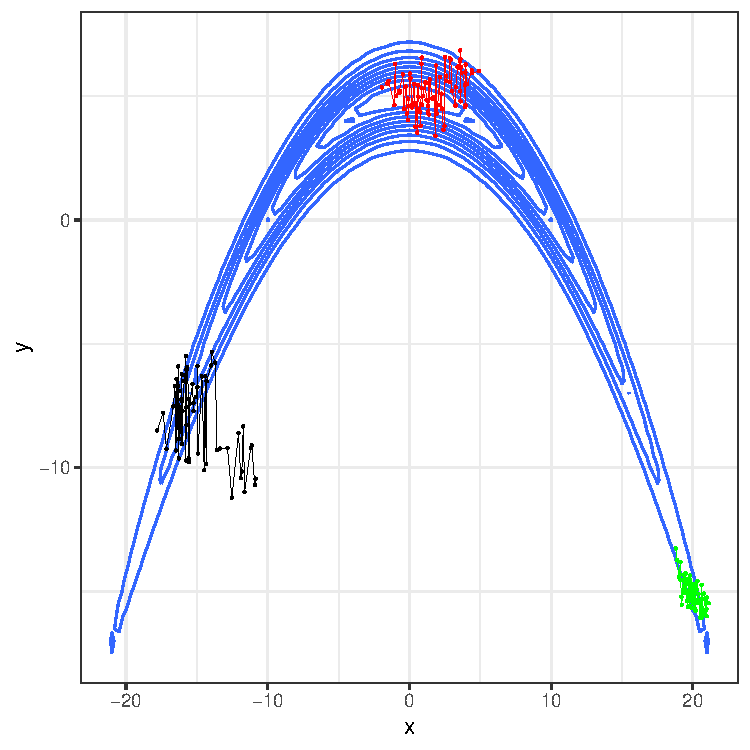
\includegraphics[width=.3\textwidth]{rule1.pdf}
            \hfill
            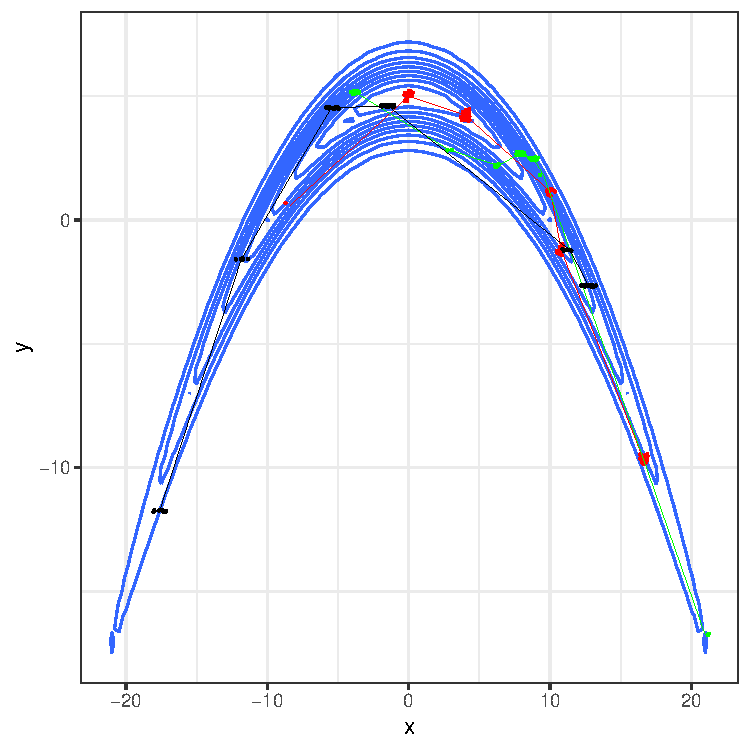
\includegraphics[width=.3\textwidth]{rule2.pdf}
            \hfill    
            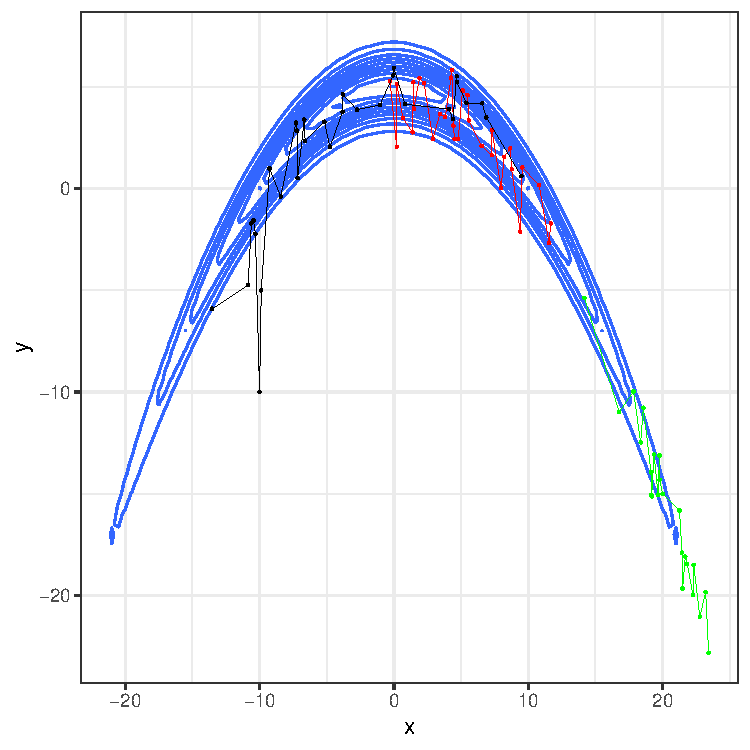
\includegraphics[width=.3\textwidth]{rule3.pdf}
            \caption{Contour plot of the distribution density with chains starting from 3 different starting points $x_1 = (0, 5), ~ x_2 = (20, -15) ~\text{and} ~x_3 = (-10, -10)$.}
            \label{fig:rules}
        \end{figure}
        \begin{table}
            \centering
            \begin{tabular}{l|l|ll}
               1 & Rej. rate & ESS (x) & ESS (y) \\ \hline
               $x_1$ & 0.171 & 13.8 & 46.2 \\
               $x_2$ & 0.344 & 3.1 & 3.0 \\
               $x_3$ & 0.298 & 1.8 & 1.6 \\
            \end{tabular}
            \hfill
            \begin{tabular}{l|l|ll}
               2 & Rej. rate & ESS (x) & ESS (y) \\ \hline
               $x_1$ & 0.937 & 13.3 & 16.3 \\ 
               $x_2$ & 0.952 & 16.4 & 20.2 \\
               $x_3$ & 0.938 & 5.1 & 12.4 \\
            \end{tabular} \\
            \vspace{10pt}
            \begin{tabular}{l|l|ll}
               3 & Rej. rate & ESS (x) & ESS (y) \\ \hline
               $x_1$ & 0.925 & 17.5 & 32.2 \\
               $x_2$ & 0.927 & 21.4 & 64.5 \\
               $x_3$ & 0.937 & 5.48 & 6.0 \\
            \end{tabular}
            \caption{Rejection rates and effective sample sizes for the tree proposal distributions.}
            \label{tab:rules}
        \end{table}
    \item D

\end{enumerate}

\end{document}